La creación de una librería en R es uno de los pilares en los que se apoya este sistema, ya que al tratarse de software de código abierto son los usuarios finales los que deben mantener de manera gratuita estas aplicaciones.\\

Para conseguir esto, los administradores de R han creado una serie de reglas y pautas lo suficientemente precisas y concisas con la finalidad de que los trabajos que se almacenen y se pongan a disposición de los clientes mantengan unos estándares de calidad lo suficientemente elevados como para que los usuarios finales confíen y así puedan utilizar este sistema. A continuación se pasan a detallar los pasos a seguir para superar estos estándares de calidad marcados por los administradores de R.
\section{Creación de un paquete local}

El primer paso para la creación de una librería en RStudio es elegir la opción \textit{Nuevo proyecto} en la pestaña \textit{Archivo} y seleccionar \textit{Nuevo directorio} y \textit{Paquete de R}. Se abrirá una ventana donde se debe colocar el nombre del paquete e indicar la dirección del disco donde situarla. Opcionalmente, se pueden adjuntar archivos de funciones ya creados para ser incluidos en el paquete. Como resultado nos encontraremos una carpeta con el nombre de nuestra librería con la siguiente estructura :\\

\begin{center}
    \centering
    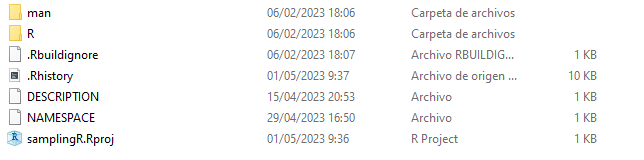
\includegraphics[scale=0.8]{img/proyecto.png}
    \captionof{figure}{Estructura de un proyecto en R.}
    \label{fig:proj}
\end{center}

Los contenidos que figuran dentro de esta carpeta de forma resumida son los siguientes:\\

\begin{itemize}[label=$\bullet$]
    \item man: carpeta donde se encuentran los ficheros de documentación de las funciones.
    \item R: carpeta donde se encuentran los archivos con extensión .R de funciones.
    \item DESCRIPTION: archivo donde se almacena información importante sobre el paquete.
    \item NAMESPACE: archivo donde se encuentran los nombres de funciones públicas al usuario y menciones sobre el uso de otras librerías de funciones en caso de requerir de sus funciones en algún momento del desarrollo.
    \item Archivo .Rproj: archivo que se usa para abrir el proyecto en una nueva sesión R.
\end{itemize}

Dependiendo de los archivos a crear pueden generarse carpetas adicionales, como explicamos en la sección dedicada a la creación de viñetas \ref{sect:3.4}
Una vez obtenida toda esta estructura, ya se podría crear un nuevo archivo de funciones dentro de la carpeta \textit{R} con el código deseado.\\

\section{Documentación de funciones}
Un apartado muy importante y  que constituye buena práctica a la hora de escribir una nueva función es la documentación. En R resulta particularmente útil definirla ya que gracias a la librería \textit{roxygen2} \cite{Roxygen2} la documentación incluida en las funciones será traducida a archivos legibles por el usuario que aparecerán en la sección \textit{Ayuda} al acceder a la documentación de dicha función, lo que facilita al usuario final  comprender mejor cuál es el objetivo de esa función. Para empezar a documentar se debe introducir el carácter \textbf{\#\textquotesingle} y utilizar un indicador adecuado, empezando con \textbf{@}, siendo los más usados los siguientes:
\\
\begin{itemize}[label=$\bullet$]
    \item title: Descripción general de la función. Indica el propósito de la función de forma breve.
    \item description: Ampliación del propósito de la función.
    \item param: Primero indica el nombre del parámetro dentro de la función y seguido de un espacio lo que representa para la función. Debe haber tantos como parámetros tenga la función.
    \item return: Indica si la función devuelve un objeto del tipo de objeto que se trata y sus contenidos si es conveniente.
    \item details: Sirve para ampliar información acerca de la función que no tenga cabida en el apartado de descripción como funcionamiento interno de la función o valores específicos de parámetros.
    \item references: En caso de querer aportar referencias teóricas sobre las que se fundamenta el código realizado.
    \item examples: Permite escribir una caso de uso de la función para referencia del usuario.
    \item importFrom: Indica que se ha hecho uso de una función externa durante el desarrollo de la función. Se utiliza escribiendo el nombre de la librería y el de la función utilizada separadas por espacios.
    \item export: Hace pública la función al usuario.
    
\end{itemize}

En ocasiones, habrá funciones de uso recurrente que se usan para comodidad a la hora de desarrollar las funciones principales, y que no es necesario ponerlas a disposición de usuario final. Es una buena práctica que estas funciones ``auxiliares'' sean documentadas como cualquier otra de nuestra librería.\\

Sin embargo, esta práctica sin más, implica su publicación al usuario general y por lo tanto aparecerán en el manual y serán accesibles por los usuarios finales. Si no queremos que esto ocurra, se deberá eliminar el indicador \textit{@export} y sustituirlo por \textit{@noRd}. De esta forma disponemos de la documentación de la función en el fichero de código, pero no aparecerá en el manual ni en la sección \textit{Ayuda}. Tampoco será accesible por el usuario final, al menos no de la forma convencional, es decir con el nombre de la función o bien con el formato \textit{librería::función}.\\

Es posible acceder a ellas utilizando tres puntos dobles, por ejemplo, \textit{samplingR:::all01list} nos permite utilizar una función auxiliar que se utiliza en este trabajo en el control de funciones para comprobar que todos los valores de todas las entradas de una lista son ceros o unos. Es un caso no deseable pero es la forma más parecida de lograr el equivalente a funciones denominadas ``privadas'' de otros lenguajes de programación.\\

\section{Librería devtools}
Devtools \cite{devtools} es una herramienta que facilita la creación y desarrollo de librerías en R. Proporciona funciones de gran utilidad y que son muy recomendables a la hora de fijar un flujo de trabajo en el desarrollo. Entre ellas podemos destacar las siguientes:\\
\begin{itemize}[label=$\bullet$, font=\bfseries]
    \item document(): traduce los comentarios en formato Roxygen2 \cite{Roxygen2} de tus funciones a archivos .md de ayuda y crea el archivo NAMESPACE actualizado. La primera vez que se ejecuta es conveniente borrar el archivo NAMESPACE creado por defecto para que escriba los nombres de tus funciones.
    
    \item check(): hace un test automatizado similar al que se ejecuta cuando realizas tu petición de subida a CRAN \cite{CRAN}. Informa de errores, avisos y notas en el paquete. También existen funciones más específicas para comprobar concretamente la documentación o si cumple los requisitos para sistemas operativos Mac o Windows. Si se utiliza RStudio también es posible hacerlo en la parte superior derecha de la interfaz, donde suele encontrarse las variables de entorno. Pestaña Build $\Rightarrow$ Check 
    
    \item build(): genera un archivo comprimido con extensión .tar.gz preparado para ser instalado o subido a CRAN \cite{CRAN}. Al igual que con \textit{check()} también existen métodos para generar el manual de uso de la librería o viñetas de las que se hablará más adelante. En la interfaz de RStudio Build $\Rightarrow$ More $\Rightarrow$ Build Source Package.
\end{itemize}

\begin{center}
    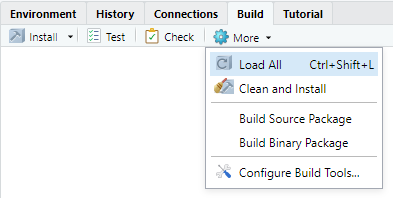
\includegraphics[scale=0.7]{img/build.png}
    \captionof{figure}{Uso de funciones de devtools desde la interfaz gráfica.}
    \label{fig:build}
\end{center}

De forma excepcional y en pocas ocasiones, es posible que al realizar check() se reciba una nota indicando que ha sido imposible comprobar la hora. Es un error que se debe a que la fecha la verifica a través de \textit{Word Clock API} \cite{worldclock} y el servicio está temporalmente inoperativo, por lo que puede ser ignorado o reintentarse más adelante.\\

\section{Creación de viñetas} \label{sect:3.4}
Generalmente, la documentación de las funciones  ayuda a dar una idea general del uso de una función específica, pero no siempre va acompañada de ejemplos de uso o esta ayuda no queda lo suficientemente clara para comprender en detalle el resultado que se pueda obtener con esas funciones. \\

Una solución útil para hacer frente al problema anterior es la creación de viñetas, las cuales se diseñan con la finalidad de mostrar la utilidad de una librería o de parte de sus funciones en su conjunto mediante la resolución de un problema propuesto. Aparecen en la ayuda del paquete antes del listado de funciones y se pueden realizar múltiples viñetas para abarcar los casos de uso más importantes para aquellas librerías de mayor extensión.\\

Para generar una viñeta se puede usar el comando \textit{usethis::use\_vignette("nombre")}. Si se trata de la primera, se creará una carpeta en la raíz del directorio del paquete con nombre \textit{vignettes}, donde se almacenarán las viñetas creadas junto a un archivo \textit{.gitignore} para evitar que los archivos creados pasen control de versiones, además de añadir las dependencias al archivo \textit{DESCRIPTION}. Dentro de la carpeta aparecerá un archivo .Rmd (es decir, se trataría de un archivo de tipo Rmarkdown) con el nombre de nuestra viñeta. En él encontramos dos bloques de código: el primero destinado a incluir los metadatos de la viñeta, como su título y forma de presentación, que puede ser como un archivo HTML, PDF, un cuaderno de trabajo similar a los cuadernos Jupiter de Python, etc. El segundo bloque incluye los ajustes predeterminados de presentación del código y sus resultados. El último simplemente realiza la llamada de nuestra librería para poder empezar a trabajar.\\


\section{Petición de subida a CRAN}
En el supuesto de que se decida subir la librería al repositorio oficial para uso general de todos los usuarios, se deberá ir al sitio web dedicado a la realización de esta acción, accesible desde la página oficial. Previamente se deberá realizar algunas modificaciones a los contenidos del paquete para poder enviarlo.\\

El archivo DESCRIPTION contiene la información principal de la librería, tal como su nombre o las personas que lo han desarrollado. Debe ser rellenado con la información pertinente. Entre sus campos encontramos: \\

\begin{itemize}[label=$\bullet$]
    \item \textit{Package}, que especifica el nombre de la librería. Éste no puede coincidir con el de ningún otro subido a CRAN con anterioridad. Los nombres son case-insensitive, por lo que, por ejemplo, samplingr no será aceptado por coincidir con el nombre de la librería de este trabajo. La forma más cómoda de buscar un nombre es ir a \textit{install} de la pestaña \textit{Packages} de RStudio  y escribir el nombre elegido, ya que con el autocompletado podrás ver los nombres con coincidencia parcial al texto introducido.
    \item \textit{Title} muestra el título que aparecerá en la página general de ayuda del paquete. Se trata de una única frase escrita en title-case, por lo que exceptuando artículos, preposiciones y similar la primera letra de las palabras debe ser mayúscula. No debe terminar en punto, ya que de lo contrario se nos avisará al subirlo al repositorio de CRAN. Tampoco conviene poner ``en R'' ya que los revisores lo consideran error por reiterativo. 
    \item \textit{Maintainer} indica la persona que lleva a cabo tareas de mantenimiento de la librería. Es importante que la información sea correcta ya que se usará para comunicar novedades sobre el estado del paquete durante el proceso de revisión y subida. Sigue el formato nombre apellido $<$correo electrónico$>$ 
    \item \textit{Authors@R} indica las personas involucradas en el desarrollo del paquete. Anteriormente se usaba un formato similar al de Maintainer, pero ahora se aconseja usar la clase \textit{person} \cite{person}. Dispone de múltiples roles para asignar a cada persona en función del trabajo realizado. 
    \item \textit{Description} amplía la información del título sobre el uso de la librería. Hay que ser moderadamente específicos con lo que realiza ya que si usas términos como \textit{diferentes funciones o varios métodos} los revisores pueden exigir elaborar sobre dichos métodos.
    \item \textit{Version} indica la versión de desarrollo de la librería. Por defecto se sitúa en 0.1.0. Es importante que cada vez que subamos una actualización del paquete al repositorio modifiquemos manualmente este valor ya que de lo contrario se detectará una coincidencia y la subida no será efectiva.
\end{itemize}

Una vez tengamos el archivo \textit{DESCRIPTION} completo, rellenaremos el formulario haciendo que el nombre y correo electrónico coincidan con los del \textit{Maintainer} y subiremos un archivo con extensión .tar.gz creado previamente con la función build(). Pasados unos minutos después del envío, llegará al correo del maintainer un mensaje de confirmación con un enlace donde se deben aceptar los términos.\\

Si nos fijamos en el segundo de estos términos, confirmamos haber realizado una comprobación de tipo check() y nos adjunta una página web. Esto se debe a que según las directrices de CRAN es necesario realizar comprobaciones como las de la función check(), pero siguiendo las normas de la próxima versión de R planeada para ser desplegada.\\

Existen dos formas de realizar estas comprobaciones. La primera es instalar R-devel, es decir la siguiente versión de R en tu ordenador para realizar ahí las comprobaciones. Este método puede resultar pesado, por lo que si entramos al enlace mencionado anteriormente veremos un lugar donde realizar comprobaciones para la versión actual, anteriores o R-devel. Solo hace falta subir el archivo con extensión .tar.gz e indicar el correo donde se quiera recibir el resultado y en cuestión de minutos llegará un enlace a un archivo tipo log donde veremos los resultados de la misma manera que realizando check() en local. En el mejor caso recibiremos solo una nota encima del maintainer, lo cual es normal ya que se trata de un recordatorio para que los maintainer comprueben en los ficheros log que la actualización ha sido solicitada por él y no otra persona, según Uwe Ligges, maintainer de CRAN.\\


\begin{figure}[H]
    \centering
    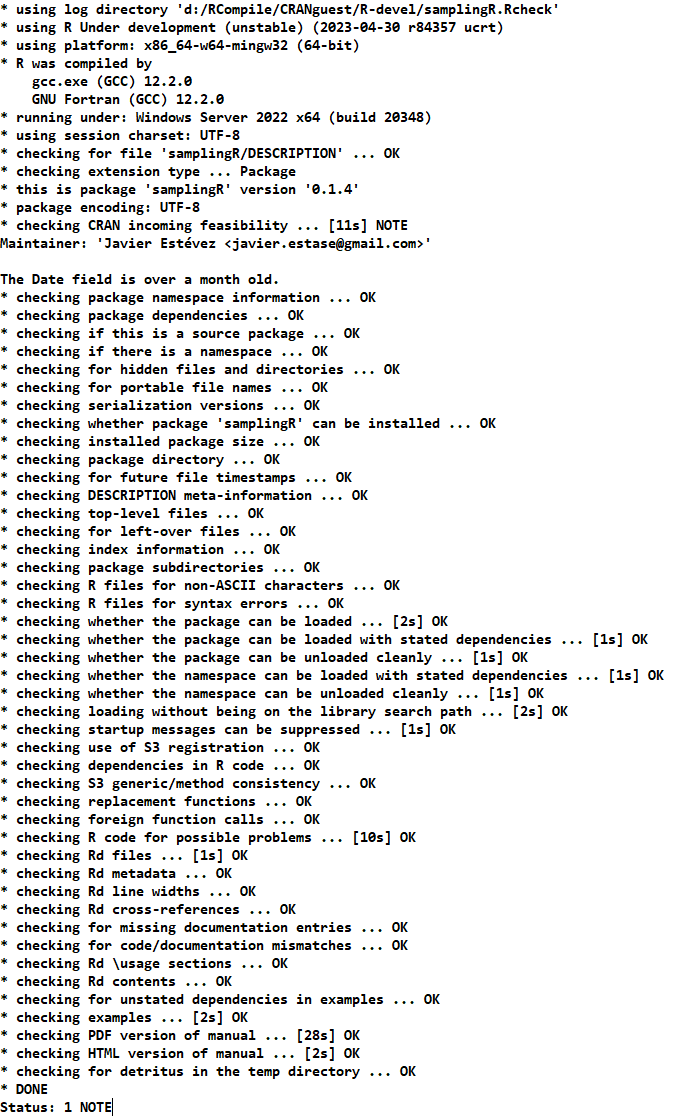
\includegraphics[scale=0.4]{./img/winbuilder.png}
    \caption{Ejemplo de resultados usando la herramienta Winbuilder.}
    \label{fig:enter-label}
\end{figure}

Una vez confirmados los términos llegará un segundo correo con los resultados de los tests automatizados. En cualquier caso, se notificará del resultado y se tendrá acceso al registro completo en un archivo tipo log. Una confusión generalizada al ver este archivo es ver una nota en el nombre del maintainer. En caso de pasar los tests se añadirá que el paquete queda pendiente de una última revisión manual. Esta última revisión será la que más se demore en la entrega de  sus resultados y es aquí donde pueden sugerir cambios que no muestre la función check() como los antes mencionados del archivo DESCRIPTION, usar TRUE y FALSE en lugar de sus homónimos T y F en el código para mejorar su comprensión o reformular descripciones de funciones que contienen ``esta función...'' por redundantes.\\

Tras recibir el visto bueno por parte de los moderadores, su respuesta será una confirmación de que el paquete se ha creado correctamente y se encuentra de camino a CRAN. Generalmente se estima un periodo de 24 horas antes de poder ser descargado por los usuarios.\\
